\chapter{The LHC and the CMS experiment}
\label{chap:detector}

\epigraph{No one can whistle a symphony. It takes a whole orchestra to play it.}{--- H.E. Luccock}

\initial{T}his chapter concerns the experimental setup. \acrshort{cern} is the organisation that manages the machines discussed and is a pioneer in the high energy physics community. As such, it will be given a short overview. The \acrlong{lhc} provides the \acrshort{cms} experiment with proton-proton collision data that is then stored, corrected, and then used by physicists for analysis. Ranging from \acrlong{sm} precision measurements, searches for new physics, the development of tools and algorithms to aid the previous two, these and much more are studied by the collaboration. \acrshort{cms} is described in detail, from its hardware and subdetectors to its data acquisition and trigger system. Special attention is given to the derivation of \acrfull{jec} in the \acrfull{l1t} as I have been a part of that effort during my PhD.


%=========================================================


\section{CERN}
\label{sec:detector_cern}

\acrshort{cern}, the European Organisation for Nuclear Research (\emph{Organisation Europ\'{e}enne pour la Recherche Nucl\'{e}aire}), is the body responsible for large scale particle and high energy physics projects in Europe. It was founded in 1954 under the \emph{Conseil Europ\'{e}en pour la Recherche Nucl\'{e}aire} (European Council for Nuclear Research), from where its acronym is derived. \acrshort{cern}'s primary site is situated in the canton of Geneva and creeps over the Franco-Swiss border. Its main purpose today is to provide physical and technological infrastructure for particle and high energy physics experiments. From large scale accelerators to extensive computing farms, \acrshort{cern} has grown into the largest laboratory for particle physics in the world. The organisation also provides a central community for the many researchers, engineers, and technicians to share ideas and collaborate effectively.

The organisation was founded by twelve European member states, the United Kingdom being one of them. It has since expanded to twenty three, encompassing most of western Europe and some of the continent's east. Many more countries from across the globe are affiliated with \acrshort{cern} in some way, providing researchers, computing resources, and more. The member states and associated members contribute to \acrshort{cern}'s budget, to the tune of 1.2 billion Swiss Francs for the year 2020~\cite{cern_budget_2020}.

Many important inventions and discoveries can be attributed to \acrshort{cern} and its personnel. Physics accomplishments include observations of weak neutral current interactions in 1973~\cite{HASERT1973121,HASERT1973138}, paving the way for the \PW~\cite{ARNISON1983103,BANNER1983476} and \PZ~\cite{Arnison:1983mk,Bagnaia:1983zx} boson discoveries with the UA1 and UA2 experiments in 1983. The number of light neutrino generations at the \acrfull{lep} in 1989~\cite{Trentadue:200667}, and direct CP violation with the NA48 experiment in 1999~\cite{Fanti_1999}, were also observed. Tim Berners-Lee and Robert Cailliau are credited with inventing the World Wide Web---the ubiquitous service for accessing the internet---in 1989/90.

\acrshort{cern} is perhaps most widely known as the home of the \acrlong{lhc}, the particle accelerator involved in the discovery of the Higgs boson~\cite{Chatrchyan:2012xdj,Aad:2012tfa}. More details regarding the machine are discussed in Chpt.~\ref{sec:detector_lhc}. But \acrshort{cern} is involved in many more undertakings. There are many fixed target experiments that use beams from the \acrshort{ps} and \acrshort{sps} such as COMPASS, that studies hadronic structure, and NA62, investigating rare decays of kaons. Experiments like ALPHA and \acrshort{aegis} use antiprotons from the Antiproton Decelerator to study antimatter in detail. The \acrshort{isolde} facility at \acrshort{cern} delivers beams of radioactive ions to perform many nuclear physics experiments.

Concern is given not just to contemporary science, but also to the physics of tomorrow. The experiments and accelerators are frequently upgraded, in particular the \acrshort{lhc} improvements documented in Chpt.~\ref{subsec:evolution_lhc}. Advanced accelerators are also being discussed, such as the \acrfull{fcc}. It would use the \acrshort{lhc} as a booster, with the final ring having a 90--100\,km circumference and up to 100\TeV centre of mass energy. Proposals for the injectants are electron-positron beams (\acrshort{fcc}-ee, $\sqrt{s} = \text{90--350}\GeV$) or proton-proton beams (\acrshort{fcc}-hh, $\sqrt{s} = \text{100}\TeV$). Each option boasts its own merits, and in an integrated scenario the former may be used as an intermediate step toward the latter.


%=========================================================


\section{The Large Hadron Collider}
\label{sec:detector_lhc}

Deep underground beneath the Franco-Swiss border lies the \acrfull{lhc}, a synchrotron particle accelerator 27\,km in circumference. As the largest machine in the world, the \acrshort{lhc} stands as a testament to the importance of fundamental science and the dedication to which it is pursued. Predominantly a proton collider, lead and xenon ions have also been injected for novel and unique studies. Four primary experiments are situated at their own interaction points where the two beams of particles are brought into contact: \acrshort{cms} (\acrlong{cms}), a general purpose detector with interests in precision measurements, searches for new physics, and many other avenues; \acrshort{atlas} (\acrlong{atlas}), a counterpart to \acrshort{cms} at its antipode on the \acrshort{lhc} ring; LHCb, designed to study the decay of \PB hadrons; and \acrshort{alice} (\acrlong{alice}), primarily studying heavy ion collisions and the quark-gluon plasma.

Four additional, smaller experiments are stationed in the \acrshort{lhc} tunnel that are much more specialised than those aforementioned: \acrshort{totem} (\acrlong{totem}) shares the \acrshort{cms} cavern with three subdetectors positioned near the beam line, performing proton structure and interaction cross section studies; LHCf shares the \acrshort{atlas} cavity and is concerned with detecting neutral pions in the forward direction to explain the origins of high energy cosmic rays; \acrshort{faser} (\acrlong{faser}) is another forward-based detector near \acrshort{atlas} and searches for light, weakly interacting particles; finally, \acrshort{moedal} (\acrlong{moedal}) is installed in proximity to LHCb and aims to detect magnetic monopoles and other exotic particles.

The technical design report for the \acrshort{lhc} can be found at Ref.~\citenum{lhc_design_report}, detailing the ring itself, infrastructure, general services, and the injector chain.


%=========================================================


\subsection{A proton's journey}  % alternative title - A big bang from a small bottle: A proton's journey to the LHC
\label{subsec:protons_journey}

A proton destined for the \acrshort{lhc} begins its journey as a hydrogen atom in a little, red bottle. Around $\text{3}\times\text{10}^{\text{14}}$ protons are supplied to each beam in the \acrshort{lhc}, with billions of refills available in this single container. Once the hydrogen atoms leave the source, they are stripped of their electrons, and [sent] to the linear accelerator LINAC2.\footnote{As of the end of Run-2, LINAC2 has been decommissioned. It has been replaced by LINAC4 in preparation for Run-3.} This is the start of a long voyage through the accelerator complex (visualised in Fig.~\ref{fig:cern_accelerator_complex}).

Given a modest boost to 50\MeV, the protons are sequentially fed from LINAC2 into the \acrfull{psb} that accelerates them further to 1.4\GeV. Another upsurge is provided once the protons travel to the \acrfull{ps}, this time to 26\GeV. Then, the final energy increase received before entering the \acrshort{lhc} comes from the \acrfull{sps}, leaving the protons at 450\GeV. Once injected into the \acrshort{lhc}, they are finally accelerated to their peak; up to 6.5\TeV from a sequence of radio frequency cavities over the course of twenty minutes. The oscillation frequency of these cavities is precisely tuned and timed to give protons the appropriate kicks and accelerate them to the desired energy. Since there is a distribution of proton energies in the beam, those that enter a cavity slightly out of time with a different energy than expected consequently become sorted into ``bunches.'' The remainder of the \acrshort{lhc} ring is used to steer the beam with the aid of over 1,200 liquid helium-cooled superconducting dipole magnets. It is also focused by almost 400 equivalently-cooled quadrupole magnets to increase the rate of proton collisions.

One beam consists of a ``train'' of up to 2,808 bunches spaced 25\,ns apart, each with 115 billion protons. Using bunches provides an advantage to the experiments at each of the interaction points. Discrete collisions take place between bunches in the opposing beams at 40\,MHz as opposed to continuous streams of protons. This allows for estimates of \gls{pileup} interactions that can be filtered out, and would otherwise introduce miscalculations of sums like \ptmiss and \HT. The data recorded by each experiment is naturally separated by the bunch crossing or \emph{event}---an event being the products of the collisions in a bunch crossing, including any \gls{pileup} interactions along with the nominal collision.

\begin{figure}[htbp]
    \centering
    \includegraphics[width=0.8\textwidth]{figures/CERN_accelerator_complex.jpg}
    \caption[A schematic of the \acrshort{cern} accelerator complex]{A schematic of the \acrshort{cern} accelerator complex. Various particles are shown from their sources to the detectors they are observed at. Figure obtained from Ref.~\citenum{cern_accelerator_complex_page}.}
    \label{fig:cern_accelerator_complex}
\end{figure}

% Describe the LHC's beam pipe, cooling? Include a couple more stats somewhere (operating/electricity power draw)? Can look in Postgraduate and CMS courses/ folder 


%=========================================================


\subsection{Luminosity}
\label{subsec:luminosity}

The \emph{\gls{luminosity}} of a particle accelerator is, along with centre of mass energy, a quantitative measure of its performance. It also often used to denote the amount of data delivered to, or collected by, the receiving detector. A full derivation of this quantity can be found in Ref.~\citenum{Herr:941318}, and as such, only a summary is given here. The \emph{instantaneous luminosity} \lumi, typically quoted in $\text{cm}^{-2}\,\text{s}^{-1}$, is defined as
\begin{equation}
    \lumi = \frac{1}{\sigma_{\mathrm{p}}} \dv{N}{t}
    \label{eq:lumi_instantaneous}
\end{equation}
where $N$ is the number of collisions and $\sigma_{\mathrm{p}}$ is the production cross section. In the \acrshort{lhc}, because many final states are possible, $\sigma_{\mathrm{p}}$ is not generally known. It can be measured, however. A recent paper from LHCb measured the extrapolated inelastic cross section (which is the important component for LHC collisions) to be $\text{75.4} \pm \text{5.4}$\,mb at \comruntwo~\cite{Aaij:2018okq}, allowing an estimate of the collision rate. For two colliding beams split into bunches with the constituents in each bunch distributed according to a gaussian profile,
\begin{equation}
    \lumi = \frac{N_1 N_2 f N_b}{4 \pi \sigma_x \sigma_y} \cdot F % \cdot H
    \label{eq:lumi_inst_head_on_colliding_beams}
\end{equation}
where $N_1$ and $N_2$ are the number of particles in a bunch in beams 1 and 2, respectively, $N_b$ is the number of bunches per beam, $f$ is the revolution frequency (11,245\,Hz for protons in the \acrshort{lhc}), and $\sigma_x$ and $\sigma_y$ are the horizontal and vertical sizes of the beam, respectively.\footnote{Add the $H$ factor from the hourglass effect and explain?}

The geometric reduction factor $F$ is unity for beams colliding head on.\footnote{Add mathematical formula for F?} However, in the \acrshort{lhc}, the beams collide at an angle known as the \emph{crossing angle} to reduce the effects of \gls{pileup}. At the start of a fill when the number of protons in the \acrshort{lhc} is at its maximum, the crossing angle at each interaction point is approximately 300\,\si{\micro\text{rad}}. As the runs progress, more protons collide and the luminosity decreases. One of measures taken to recover luminosity and keep the \acrshort{lhc} as efficient as possible is to reduce the crossing angle. By the end of the fill, it can be as small as 240\,\si{\micro\text{rad}}.

% For mathematical formula for F, see \url{https://espace.cern.ch/DG-DAT/public/Springer_Volume%20I21C/9_Lamont/luminosity/Luminosity%20Optimization.pdf}

The instantaneous luminosity can be increased further by the inclusion of more bunches per beam, decreasing the size of a beam through improved quadrupole magnets, and by reducing the crossing angle. Tuning these parameters led the \acrshort{lhc} to reach is design luminosity of 10$^{34}\percms$ in 2016. It had more than doubled by the end of Run-2.

Integrating the the instantaneous luminosity over a period of time yields the \emph{integrated luminosity} \intlumi:
\begin{equation}
    \intlumi = \int \lumi \dd{t}
    \label{eq:lumi_integrated}
\end{equation}
These values are often quoted by experiments in units of ``inverse femtobarn'' ($\text{fb}^{-1}$) as an indicator of the amount of collision data collected. A ``barn'' is a unit equal to 10$^{-28}$\,m$^2$ and colloquially used to express cross sectional area in nuclear and particle physics. Thus its reciprocal, the same units as integrated luminosity, gives a good sense of scale that relates cross sections of individual processes to the total amount of data. Tab.~\ref{tab:lumis_lhc_cms} gives the integrated luminosities over Run-2 delivered by the LHC and collected by CMS. Taking 137.19\,\fbinv from this table, and assuming the inelastic \pp cross section above gives an estimate of 10$^{16}$ collisions recorded by \acrshort{cms} over Run-2 (excluding \gls{pileup} interactions).


%=========================================================


\subsection{Pileup}
\label{subsec:pileup}

At the high instantaneous luminosity of the \acrshort{lhc}, multiple interactions per bunch crossing---known as \emph{\gls{pileup}}---are frequent. The expected, or nominal, number of collisions per bunch crossing is one, but because of all the factors that increase the luminosity, many ``softer'' collisions also take place. \Gls{pileup} interactions can produce many low-\pt objects, and near-collinear to the beam (detecting particles in this region is essential for some analyses). These additional objects can contaminate the reconstruction of the final state from the nominal collision, and as such affect the direction and magnitude of the \ptvecmiss. When one aims to increase the luminosity to collect more data, the more severe pollution from \gls{pileup} is an inevitable consequence. The distribution of \gls{pileup} events in \acrshort{cms} during Run-2 can be seen in Fig.~\ref{fig:detector_cms_pileup}.

There are strategies in place in the LHC and the anchored experiments to mitigate \gls{pileup}. Introducing, or increasing, a crossing angle between the beams reduces the effect. Decreasing the crossing angle increases the overlap between bunches at each intersection---since they have a non-negligible length---leading to more collisions. Track reconstruction algorithms are very efficient at connecting particles to their primary vertices, and therefore particles originating from \gls{pileup} vertices can be identified and removed~\cite{Chatrchyan:2014fea,Aaboud:2017all}. At \acrshort{cms}, various methods are available in the calorimeter triggers to subtract the effects of \gls{pileup}.

\begin{figure}[htbp]
    \centering
    \includegraphics[width=0.75\textwidth]{figures/pileup_allYears_run2.pdf}
    \caption[The average number of pileup interactions per bunch crossing at CMS during Run-2 of the LHC]{The average number of \gls{pileup} interactions per bunch crossing at \acrshort{cms} during Run-2 of the LHC. Figure obtained from Ref.~\citenum{cmslumitwikipage}.}
    \label{fig:detector_cms_pileup}
\end{figure}


%=========================================================


\subsection{Evolution of the LHC}
\label{subsec:evolution_lhc}

The \acrshort{lhc} began operating in 2010 at a centre of mass energy of $\sqrt{s} = \text{7}\TeV$; 3.5\TeV per beam. A modest increase to 8\TeV was achieved by the end of Run-1 in 2013. Long Shutdown 1 then commenced where maintenance work was carried out, and upgrades to the accelerator and experiments were performed. Notably, the superconducting magnets were improved to safely handle much more energetic beams.

The LHC resumed operation in 2015, marking the start of Run-2 and further pushing the frontiers of high energy physics with a centre of mass energy of \comruntwo. While valuable data was taken that year, it was not until 2016 when substantial datasets were amassed. Therefore, when analysts refer to the ``full Run-2 dataset,'' they typically do not include data from 2015. It requires as much care as the other years with respect to implementing corrections and addressing systematic uncertainties, and so on, for only a very small gain in integrated luminosity. Run-2 ended in 2018 with---omitting the 2015 dataset---158.64\fbinv of \pp collisions delivered, 146.45\fbinv of which were recorded by \acrshort{cms} who certified 137.19\fbinv suitable for analysis~\cite{cmslumitwikipage,cmslumipogpage}. A breakdown by year is presented in Tab.~\ref{tab:lumis_lhc_cms}\footnote{Maybe add Run-1 column(s)? One for 7\TeV (or 2011) and one for 8\TeV (or 2012)? Though, it does risk becoming too cluttered.} with a visual chart in Fig.~\ref{fig:detector_cms_lumi}.\footnote{As I'm considering with the table, should I replace this figure with the one that also includes Run-1? But then there are lots of lines and things can look less clean.} By comparison, the \acrshort{lhc} delivered only 6.2\fbinv at 7\TeV and 23.3\fbinv at 8\TeV over the course of Run-1.

\begin{table}[htbp]
    \centering
    \begin{tabular}{lccccc}
        \hline
        Integrated luminosity & 2015 & 2016 & 2017 & 2018 & Full Run-2 \\ \hline
        Delivered by \acrshort{lhc} (\fbinv) & 4.21 & 40.99 & 49.79 & 67.86 & 162.85 \\
        Recorded by \acrshort{cms} (\fbinv) & 3.80 & 37.80 & 44.98 & 63.67 & 150.25 \\
        Certified by \acrshort{cms} (\fbinv) & 2.26 & 35.92 & 41.53 & 59.74 & 139.45 \\
        \hline
    \end{tabular}
    \caption[The integrated luminosity delivered by the LHC during Run-2 which were recorded and certified by CMS]{The integrated luminosity delivered by the \acrshort{lhc} during Run-2 which were recorded and certified by \acrshort{cms}. Typically, only the 2016$-$18 datasets are analysed since 2015 accrued little data compared to the other years. Numbers obtained from Refs.~\citenum{cmslumitwikipage,cmslumipogpage}.}
    \label{tab:lumis_lhc_cms}
\end{table}

\begin{figure}[htbp]
    \centering
    \includegraphics[width=0.75\textwidth]{figures/int_lumi_cumulative_pp_2_run2.pdf}
    \caption[The integrated luminosity of \pp collision data delivered to CMS during Run-2 of the LHC]{The integrated luminosity of \pp collision data delivered to \acrshort{cms} during Run-2 of the LHC. Figure obtained from Ref.~\citenum{cmslumitwikipage}.}
    \label{fig:detector_cms_lumi}
\end{figure}

In addition to the upgrades that have so far been performed, a much grander change is on the horizon. In 2027, the \acrfull{hllhc} improvements are set to be introduced with the primary purpose of increasing the luminosity by up to a factor of ten: more powerful magnets for focusing the beam, crab cavities for increasing the bunch overlap area, shielding and more radiation-resistant components, an upgrade to many of the boosters in the accelerator complex, and much more. A summary of the important parameters at three stages of the LHC's life is given in Tab.~\ref{tab:lhc_specs}.\footnote{Should I add a column for the Tevatron, as a comparison to/sense of scale for the LHC's numbers? Or maybe discuss the Tevatron qualitatively somewhere.}

\begin{table}[htbp]
    \centering
    \begin{tabular}{lccc}
        \hline
        Parameter & End of Run-2 & \acrshort{hllhc} & Design \\ \hline
        Beam energy (\TeVns) & 6.5 & 7 & 7 \\
        Bunches per beam & 2,556 & 2,748 & 2,808 \\  % bunches per beam in Run-2 from https://home.cern/news/news/accelerators/lhc-report-lhc-full
        Protons per bunch & $\text{1.5} \times \text{10}^{\text{11}}$ & $\text{2.2} \times \text{10}^{\text{11}}$ & $\text{1.5} \times \text{10}^{\text{11}}$ \\
        Crossing angle (\si{\micro\text{rad}}) & 300 & 590 & 285 \\
        Instantaneous luminosity ($\text{cm}^{-2}\text{s}^{-1}$) & $\text{2.1} \times \text{10}^{\text{34}}$ & $\text{7.2} \times \text{10}^{\text{34}}$ * & $\text{1.0} \times \text{10}^{\text{34}}$ \\  % peak lumi in Run-2 from https://home.cern/news/news/accelerators/lhc-report-lhc-full
        Integrated luminosity per year (\fbinv) & 68 & 250 & 40 \\  % 40 fb-1 for design integrated lumi using instantaneous lumi of 1e34
        Average \gls{pileup} per bunch crossing & 34 & 140 & 27 \\
        \hline
    \end{tabular}
    \caption[Some of the important parameters defining the performance of the LHC at the end of Run-2, for the High-Luminosity LHC, and the design specification]{Some of the important parameters defining the performance of the \acrshort{lhc} at the end of Run-2, for the \acrlong{hllhc}, and the design specification. Several values in this table were obtained from Refs.~\citenum{Benedikt:2112115,Apollinari:2017cqg}.

    * Does not account for the large increase to virtual luminosity from the introduction of crab cavities.}
    \label{tab:lhc_specs}
\end{table}


%=========================================================


\section{The CMS experiment}
\label{sec:detector_cms_exp}

The \acrfull{cms} collaboration was formed in 1992 with a letter of intent circulated to the high energy physics community for a general purpose detector to be built at the \acrshort{lhc}~\cite{DellaNegra:290808}. Though its emphasis was the detection of the Higgs boson, the myriad avenues for which physics could be studied was also acknowledged. Just under five hundred people from sixty two institutes were part of the original letter. At the time of writing over five thousand physicists, engineers, technical and administrative staff, and students, spanning over two hundred institutes in fifty countries, comprise the collaboration. Working tirelessly in harmony, with ingenuity, cooperation, and a drive for exploring the frontiers of particle physics, almost one thousand publications have been produced with data collected by the experiment. These range from exotic/\acrshort{bsm} searches, \acrlong{sm} precision measurements, \PB-physics, top quark physics, heavy ions, and more. This wide scope of topics cements \acrshort{cms} as a versatile and world-leading detector, and collaboration as a whole.

% Can look in Postgraduate and CMS courses/ folder for more info.


%=========================================================


\subsection{The CMS detector}
\label{subsec:cms_detector_itself}

The machine itself---aptly named the \acrshort{cms} Detector---lives a hundred metres underground at Interaction Point 5, just outside the town of Cessy in France. Constructed over several years, the detector was separated into fifteen sections. Each was built on the surface and lowered into the experimental cavern with an incredibly small tolerance of a few centimetres. Here, they were joined together to assemble the 14,000 tonne goliath. The finished detector is a hermetic cylinder enclosing the \acrshort{lhc} beam pipe, measuring 21\,m in length (plus a little extra from the bolt-on forward calorimeters) and 15\,m in diameter. Its etymology stems from how \emph{compact} (relatively speaking) the detector is since its weight is twice that of \acrshort{atlas} in only one sixth of the volume, it has a subsystem dedicated to detecting \emph{muons}, and a \emph{solenoid} is used to generate the magnetic field.

A kaleidoscope through we which see the subatomic, \acrshort{cms} is designed to detect all manner of particles as accurately as possible. To accomplish this, the detector is divided into four major subsystems (or subdetectors): the silicon tracker, the \acrfull{ecal}, the \acrfull{hcal}, and the muon chambers. These are each explained in more detail below, with a graphic of the entire detector presented in Fig.~\ref{fig:detector_cms_cutaway} and a transverse slice through it in Fig.~\ref{fig:detector_cms_transverse}.

\begin{figure}[htbp]
    \centering
    \includegraphics[width=0.9\textwidth]{figures/cms_160312_06.pdf}
    \caption[A cutaway diagram of the CMS detector with all of the principal components labelled. This detector configuration was used for the 2017--18 data taking years]{A cutaway diagram of the \acrshort{cms} detector with all of the principal components labelled. This detector configuration was used for the 2017--18 data taking years, where the coverage of the pixel detectors in the silicon tracker were upgraded. Image taken from Ref.~\citenum{Sakuma:2665537}.}
    \label{fig:detector_cms_cutaway}
\end{figure}


%=========================================================


\subsubsection{Geometry}
\label{subsubsec:geometry}

Collider physics tends to use certain conventions when describing the positions of particles in a detector. The azimuthal angle $\phi$ is the same variable as in cylindrical coordinates, i.e., the angle subtended from the 0$^{\circ}$ direction on the polar axis to the particle's position, with a range $[-\pi, \pi]$. Pseudorapidity, denoted by $\eta$, is a coordinate that describes the angle between a particle and the longitudinal axis of the detector (the beam line):
\begin{equation}
    \eta = -\ln \left[ \tan(\frac{\theta}{2}) \right]
    \label{eq:eta_def}
\end{equation}
where $\theta$ is the angle between the particle's three-momentum $\vec{p}$ and the positive direction of the beam axis. So as $\theta \rightarrow \text{0}^{\circ}$ (the beam line), $\eta \rightarrow \infty$. Generally, particles with large $\eta$ escape the detector which is why forward calorimeters are in place. The transverse momentum of a particle can be found with $\pt = \abs{\vec{p}} / \cosh \eta$. The convention in hadron colliders is to use $\eta$ over the rapidity $y$, where the latter is Lorentz invariant and tends to the former in the limit $\abs{\vec{p}} \gg m$. However, in cases such as jet clustering, soft particles are included and so $y$ is defined:
\begin{equation}
    y = \frac{1}{2} \ln (\frac{ E + p_{\mathrm{L}} }{ E - p_{\mathrm{L}} })
    \label{eq:rapidity_def}
\end{equation}

where $p_{\mathrm{L}}$ is the longitudinal component of the momentum. The subdetectors of \acrshort{cms} are nominally separated into several sections dependent on their geometry or layout, and it is useful to divide them into $\eta$ ranges to demonstrate their coverage. ``Barrel'' sections are cylindrical around the beam line while ``end caps'' are usually discs or plates perpendicular to it. The following subsections describe them in detail. One quadrant of \acrshort{cms} showing the $\eta$ divisions can be seen in Fig.~\ref{fig:cms_eta_bounds}.

The distance between two objects can be found with the variable $\Delta R$:
\begin{equation}
\Delta R = \sqrt{(\Delta \eta)^2 + (\Delta \phi)^2}
\label{eq:delta_r}
\end{equation}

It is often used as a distance parameter in jet clustering, or between individual objects in highly-boosted decays.

\begin{figure}[htbp]
    \centering
    \includegraphics[width=0.75\textwidth]{figures/cms_eta_ranges.pdf}
    \caption[A quadrant of the CMS detector illustrating the main subsystems with their radius $R$, longitudinal distance $z$, and pseudorapidity $\eta$ from the interaction point]{A quadrant of the \acrshort{cms} detector illustrating the main subsystems with their radius $R$, longitudinal distance $z$, and pseudorapidity $\eta$ from the interaction point. The grey box at $\text{3} < \abseta < \text{5}$ and $\text{11} < z < \text{12}$\,m is the hadron forward calorimeter. Figure taken from Ref.~\citenum{cms_dp_end_of_run2}.}
    \label{fig:cms_eta_bounds}
\end{figure}


%=========================================================


\subsubsection{The tracker}
\label{subsubsec:cms_tracker}

When a collision occurs, the ejected particles first encounter the silicon tracker that extends from 4\,cm to just under 1\,m in radius~\cite{Karimäki:368412,CERN-LHCC-2000-016}. Longitudinally, it is confined to $\abseta < \text{2.5}$, known as the ``central region.'' The barrel and end cap sections are bound by $\abseta \lesssim \text{1.6}$ and $\text{1.6} \lesssim \abseta < \text{2.5}$, respectively.

Consisting of tens of millions of pixels and microstrips, the positions of particles can be recorded to within 10\,\si{\micro}m. Initially, the pixel detector was arranged in three layers, covering 1\,m$^2$ and consisting of 66 million channels. It was upgraded for the 2017--18 run period to introduce a fourth layer, increasing its coverage to 1.9\,m$^2$ with 124 million channels. The many layers of strip modules enclose the pixel detector. Since the tracker is the closest subsystem to the interaction point, the components must be extremely radiation-tolerant to withstand the bombardment of particles pummelling them every collision.

The hit is registered by a pixel or strip via electron-hole pairs created by the ionisation caused from a particle interacting with the silicon. An electric field within the sensor separates them and they drift toward the electrodes at the boundaries. The activity is then read out, where pixels record electrons and strips record holes.

Track-finding algorithms use pattern recognition to determine whether the hits from multiple layers in the tracker can be correlated and reconstructed to originate from individual particles. Each is suited to different types of track, \pt threshold, and location. Vertex reconstruction algorithms are employed to determine the primary vertex. Any secondary vertices transverse (for example, in \glspl{bjet}) or longitudinal (\gls{pileup}) to the beam line may also be distinguished. The momentum of particles can be measured from the curvature of the track from the magnetic field induced by the solenoid (see Chpt.~\ref{subsubsec:cms_magnet_muons}).\footnote{Should I mention something about resolution as well?} One of the algorithms, the \acrfull{gsf} method, is used extensively in the \acrshort{hlt} for triggering on electrons and photons~\cite{Anuar_2015}.


%=========================================================


\subsubsection{The ECAL}
\label{subsubsec:cms_ecal}

After the tracker, the particles can interact with the \acrshort{ecal}~\cite{CERN-LHCC-97-033,Bloch:581342}. The 76,000 lead-tungstate crystals scintillate the incoming light, where the attached avalanche photodiodes record energy deposits in the barrel region ($\abseta < \text{1.48}$) belonging to charged particles. Vacuum phototriodes are instead glued to the crystals in the end caps ($\text{1.48} < \abseta < \text{2.96}$) as they are subject to higher radiation doses. A lead-silicon preshower detector precedes the end cap crystals to improve spatial resolution and discrimination of multiple particles. Electronics for groups of $\text{5}\times\text{5}$ crystals (the \acrshort{ecal} component of a ``trigger tower'') read out the data and deliver it to the trigger system (see Chpt.~\ref{subsec:cms_recording_data}).

The \acrshort{ecal} is designed to identify charged particles, primarily electrons and photons. The $\HepProcess{\PH \to \Pphoton\Pphoton}$ and $\HepProcess{\PH \to \PZ\PZ \to 4\Plepton}$ processes were kept in mind, as an ardent focus was on discovering the Higgs boson. These particles are usually stopped entirely in the subdetector. Muons and tau leptons ($\Ptau$), however, usually penetrate farther. Measuring the energy of electrons and photons is performed as follows:
\begin{equation}
    E_{\Pe, \Pphoton} = G(\eta) \cdot F_{\Pe, \Pphoton} \cdot \sum_i A_i S_i(t) c_i
    \label{eq:ecal_energy}
\end{equation}
where $G$ is the global energy scale, $F$ is the cluster correction (as several hits in a cluster can belong to one object, especially when they electromagnetically shower), $A$ is the amplitude of the pulse from the readout electronics, $S$ is the time-dependent response correction from the laser monitoring system that measures the crystal transparency, and $c$ an intercalibration correction that accounts for the non-uniform response of the crystals and photodetectors.\footnote{Should I mention something about energy resolution as well?} Charged hadrons, muons and taus only deposit a sliver of energy in the \acrshort{ecal}, and so information from the other subdetectors is required in their cases. 


%=========================================================


\subsubsection{The HCAL}
\label{subsubsec:cms_hcal}

Hadronic particles propagate past the \acrshort{ecal} into the \acrshort{hcal}~\cite{CERN-LHCC-97-031}. The barrel ($\abseta < \text{1.30}$) and end cap ($\text{1.30} < \abseta < \text{2.96}$) regions both consist of brass absorber\footnote{Famously, a large component of the brass used to build the end caps came from over 1 million decommissioned Russian naval artillery shells left over from World War II.} and plastic scintillator with wavelength-shifting fibre. Arranged in wedges in the barrel and discs in the end cap, hybrid photodiodes record the signal in either case. This yields 7,000 detection channels. Due to colour confinement, hadrons are much more prone to showering than charged leptons. Additional scintillator tiles are placed outside the yoke of solenoid in the barrel region to capture the tails of these showers.

Unlike the \acrshort{ecal} which only covers the barrel and end cap, the \acrshort{hcal} also has a component in the forward region of the detector: the \acrfull{hf}. Composed of steel absorber and quartz fibres with 1,000 channels on each side, and occupying $\text{2.96} < \abseta < \text{5.19}$,\footnote{I'm not entirely sure what the bounds of the \acrshort{hf} are. Literature seems to define it as $3.0 < \abseta < 5.0$, but in the \acrshort{jec} the edge of the final \abseta bin is 5.191.} it is designed to detect particles with trajectories close to the beam line. The additional function of measuring the luminosity delivered to, and collected by, the experiment is also served. Cherenkov light kindled in the fibres is funnelled into photomultiplier tubes that collect the signal. Particles that enter the \acrshort{hf} are usually not supplemented by tracker or \acrshort{ecal} information. As such, the energy and momentum of particles can be determined only by the subdetector.

Each cell of the \acrshort{hcal} maps onto a given number of \acrshort{ecal} crystals, forming trigger towers or calorimeter towers that are important when collecting data (see Chpt.~\ref{subsec:cms_recording_data}). The towers project mostly-radially from the interaction point. Their granularity is greatest at low $\eta$, and decreases with increasing $\eta$. Information from both subdetectors is used to identify \glspl{jet}, muons, and taus, as well as any electrons or photons that penetrate through the \acrshort{ecal}. Readout electronics are mounted to the various components of the \acrshort{hcal} to deliver to the trigger system. The response and transparency of modules is corrected for in a similar way to the \acrshort{ecal}, as is intercalibration.


%=========================================================


\subsubsection{The magnet and muon chambers}
\label{subsubsec:cms_magnet_muons}

The three subsystems described above are encased in a massive superconducting solenoid~\cite{CERN-LHCC-97-010}, making up 12,500 of the 14,000 tonne detector. It generates a magnetic field of 3.8\,T and $\text{2.4} \times \text{10}^9$\,J of energy, making it the largest store of energy in the world for a single magnet. The field allows for the transverse momentum of a charged particle to be precisely measured, since the field propels it into a circular orbit. The magnetic force $qvB$ exerted is equal to the centripetal force $mv^2/r$, and therefore the radius of the orbit is proportional to the momentum.

An iron return yoke interspersed with the muon chambers~\cite{Layter:343814} constitute the rest of the detector, extending from a radius of around 3\,m to 7.5\,m. The iron yoke confines the magnetic field to the volume of the detector and provides a 2\,T field in the opposite direction to that found farther inward. Since muons are much heavier than electrons and have high \pt, they penetrate farther than the bounds of the \acrshort{ecal} and deposit little energy in the process. The final states of several interesting decays include muons, such as with the Higgs boson. Consequently, constructing a dedicated subdetector is therefore essential.

There are four muon ``stations,'' as can be seen by the orange strips in Fig.~\ref{fig:detector_cms_transverse}, separated by layers of the return yoke. 480 resistive plate chambers and 250 drift tubes reside in the central barrel region of $\abseta < \text{1.2}$. The end caps are populated with 576 resistive plate chambers, complemented by 540 cathode strip chambers. Its limits are $\text{0.9} < \abseta < \text{2.4}$, though the resistive plate chambers terminate at $\abseta = \text{1.9}$. Like many of \acrshort{cms}' subdetector components, they are designed parallel and perpendicular to the beam line, not according to $\eta$. With such large segments at high radius in the muon chambers, a small overlap is therefore present. This $\text{0.9} < \abseta < \text{1.2}$ sector is sometimes referred to as the ``overlap region.'' The pseudorapidity range of the muon chambers' end cap is restricted compared to the \acrshort{ecal} and \acrshort{hcal} to (mostly) align with the tracker, and the steel that surrounds the structure takes up the remainder of the $\eta$ that the former two occupy.

All of the detectors in the muon chambers take advantage of gaseous ionisation, as it is much less expensive than the silicon used in the tracker while still providing excellent resolution. If a muon enters a cell in a drift tube or cathode strip chamber, its position can be measured by the length of time taken for the gas it ionises to drift to the anode wire of said cell in the presence of a strong electric field. The latter can additionally utilise the induced charge on the cathode strips for improved spatial resolution. The resistive plate chambers work on a similar principle, but use parallel plate capacitors and are predominantly used for timing purposes when the data is sent to the trigger system. To measure the momentum of the muons, information from both the tracker and muon detector are used where possible.\footnote{Maybe mention the upgrades done between Run-1 and Run-2 (each subsystem), and possibly even the planned upgrades for Run-3 and Phase-2.}

\begin{figure}[htbp]
    \centering
    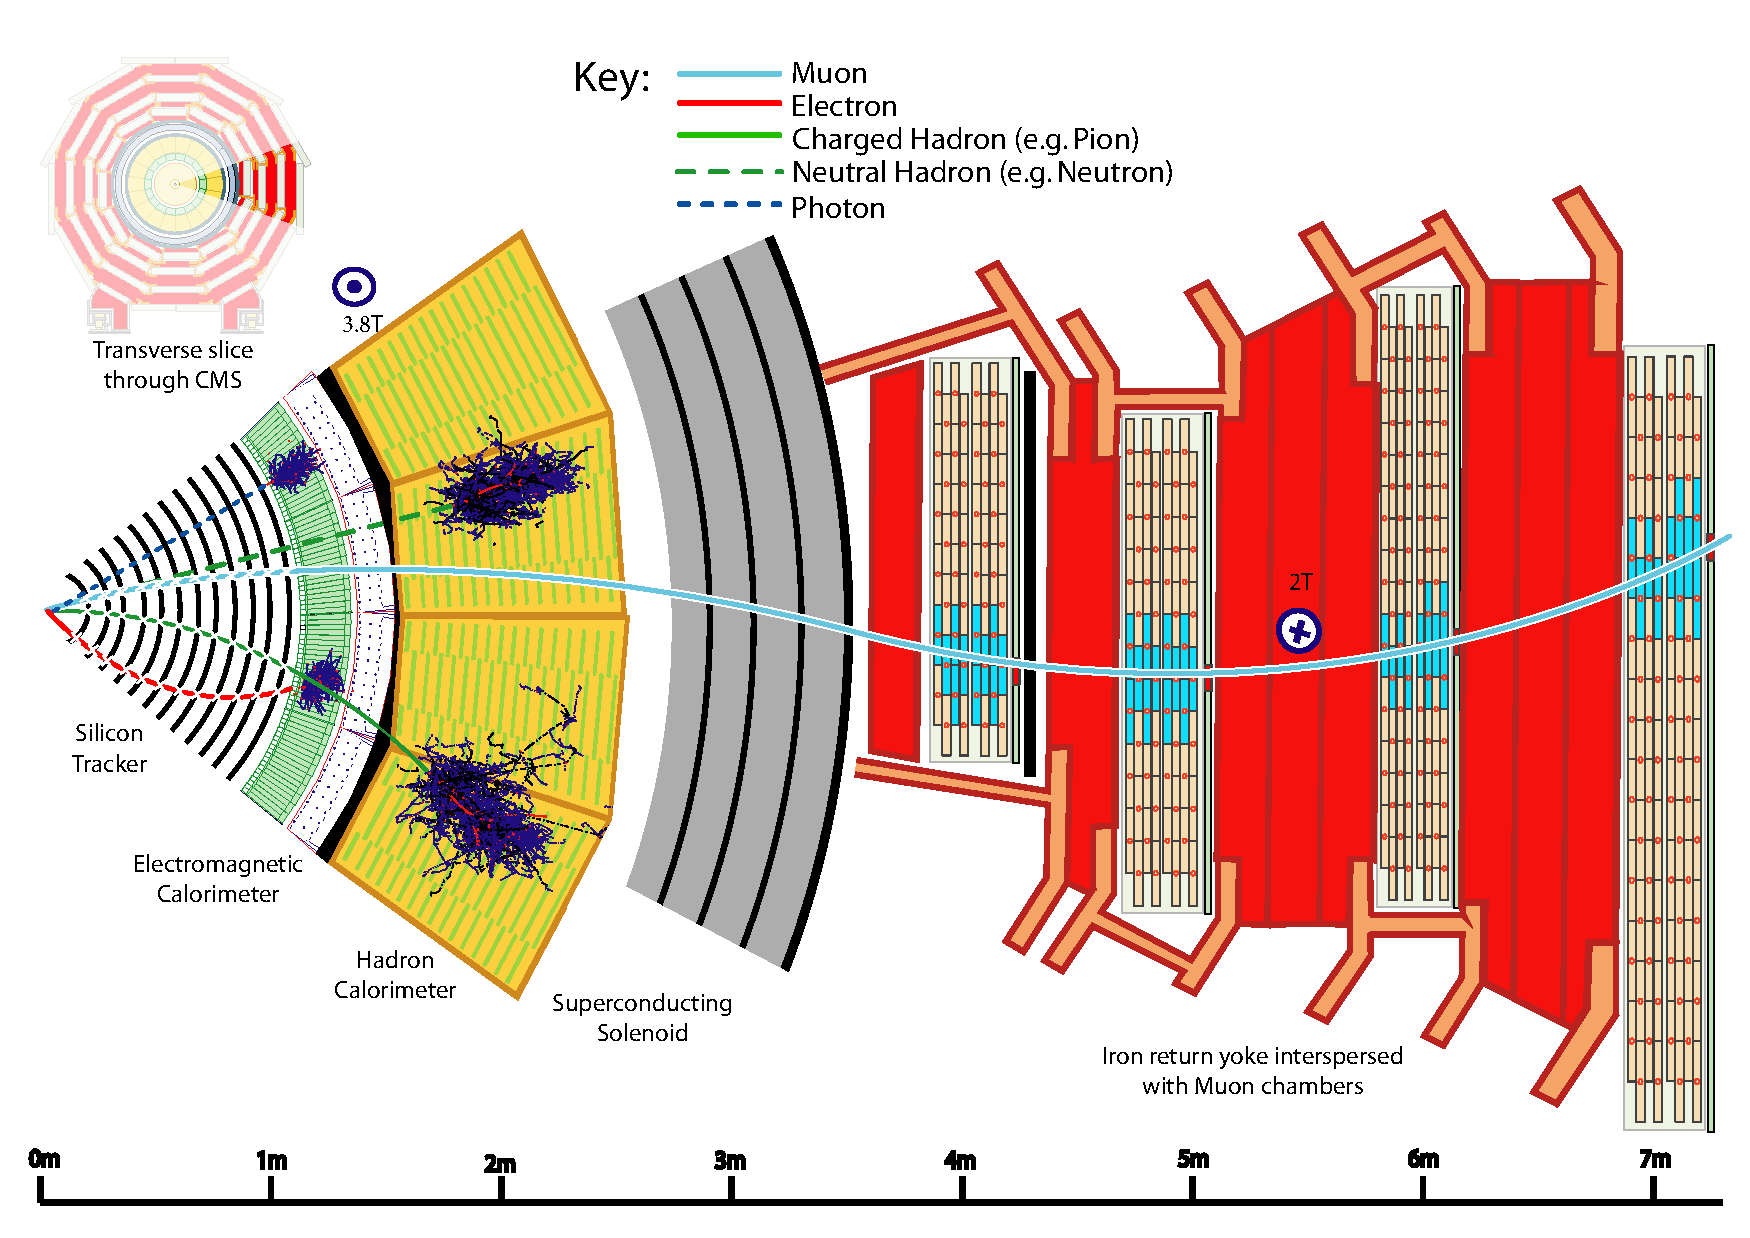
\includegraphics[width=0.75\textwidth]{figures/Transverse_slice_CMS.pdf}
    \caption[A transverse slice through the barrel section of the CMS detector with the main subsystems and components visible]{A transverse slice through the barrel section of the \acrshort{cms} detector with the main subsystems and components visible. Several particles produced at the primary vertex and their interactions with the detector are also depicted. Figure obtained from Ref.~\citenum{CMS-PRF-14-001}.}
    \label{fig:detector_cms_transverse}
\end{figure}

% Phase-1 upgrade TDRs: HCAL \cite{Mans:1481837}, pixels \cite{Dominguez:1481838}, L1T \cite{Tapper:1556311}.
% Phase-2 upgrade TDRs: tracker \cite{Collaboration:2272264}, barrel calorimeters \cite{Collaboration:2283187}, end cap calorimeters \cite{Collaboration:2293646}, muon detectors \cite{Collaboration:2283189}, L1T \cite{Collaboration:2283192}, DAQ \cite{Collaboration:2283193}.
% Can look at CMS detector section in CMS papers for an overview of things. Give more detail where appropriate.


%=========================================================


\subsection{Data acquisition and triggering}
\label{subsec:cms_recording_data}

With the enormous collision rate at the \acrshort{cms} interaction point, acquiring data requires some thought and ingenuity. Today's electronics cannot handle the bandwidth from recording every single collision, $\order{\text{1\,petabyte/s}}$. As such, a \emph{trigger} is used to select the events that may be of use to analysers. In \acrshort{cms}, a two stage trigger~\cite{Bayatyan:706847} is used: the \acrfull{l1t}, implemented in the detector hardware; and the \acrfull{hlt}~\cite{Cittolin:578006}, a software farm to further reduce the events selected at \acrlong{l1}. The trigger is part of the larger \acrfull{daq} system. An intricate network of custom electronics and commercial processors---a union of hardware, firmware, and software---are interconnected by multi-gigabit links to record the products of the highest-energy manmade collisions on Earth.


%=========================================================


\subsubsection{The Level-1 Trigger}
\label{subsubsec:detector_l1t}

The \acrlong{l1t} is a set of algorithms (a trigger menu)\footnote{Do I need to say that different menus are used throughout the data-taking periods and for different injectants (heavy ions, etc.)?} implemented in custom hardware designed to reduce the event rate from 40\,MHz to a maximum of 100\,kHz. FPGA and ASIC chips contain the algorithms in firmware, with timing systems synchronised with the \acrshort{lhc} clock. When a collision occurs, particles interact with the detector and hits are registered by the components.

Coarsely-segmented data is read out from the \acrshort{ecal} and \acrshort{hcal} through a two-layer Calorimeter Trigger. These are arrays of custom processors located at Point 5. Layer-1 receives the calorimeter data from upwards of one thousand fibre optic links, each with multi-gigabit bandwidths. The information from the two subsystems are combined into calorimeter towers, and some simple position- and energy-dependent calibrations are applied.\footnote{Mention something about trigger primitives here?} The data from Layer-1 is then transmitted to Layer-2, again over many high-bandwidth optical links. Here, physics object candidates are identified (\glspl{jet}, \Pe, \Pphoton, \Ptau).\footnote{An overview of the latest Run-2 algorithms for object identification can be found in Ref.~\citenum{Zabi_2017}.} Additional calibrations are applied to them (for example, in Chpt.~\ref{subsec:detector_jecs}), and simple \gls{pileup} subtraction is performed.\footnote{Do I need to describe in detail how jets are formed? Jet seed, chunky donut PU subtraction, etc... Since it may be relevant for \acrshort{jec}.} Energy sums are also calculated at this stage, such as \etmiss, \HT, and \mht.

In parallel, the various subdetectors in the muon chambers pass information through successive stages, and is then combined with some of the calorimeter information in a sorting/merging/isolation layer. The output from this layer is combined with the remaining information within Layer-2 in the Global Trigger, a series of \si{\micro}TCA boards with FPGAs. The trigger menu lives here, and all of the information gathered---object candidates, energy sums, beam conditions---is provided to it. These triggers may be dependent on the presence a single object or the number of objects of a single class (e.g., one muon, two \glspl{jet}), multiple classes of object (cross triggers), the energy sums, the topologies of objects, and more. The latency given to make a decision on whether to keep or reject an event is 4\,\si{\micro}s.\footnote{Mention pre--scaling of triggers, and that as \lumi decreases over a fill, the pre--scales change?} A diagram of this data flow is given in Fig.~\ref{fig:cms_l1t_data_flow}.

\begin{figure}[htbp]
    \centering
    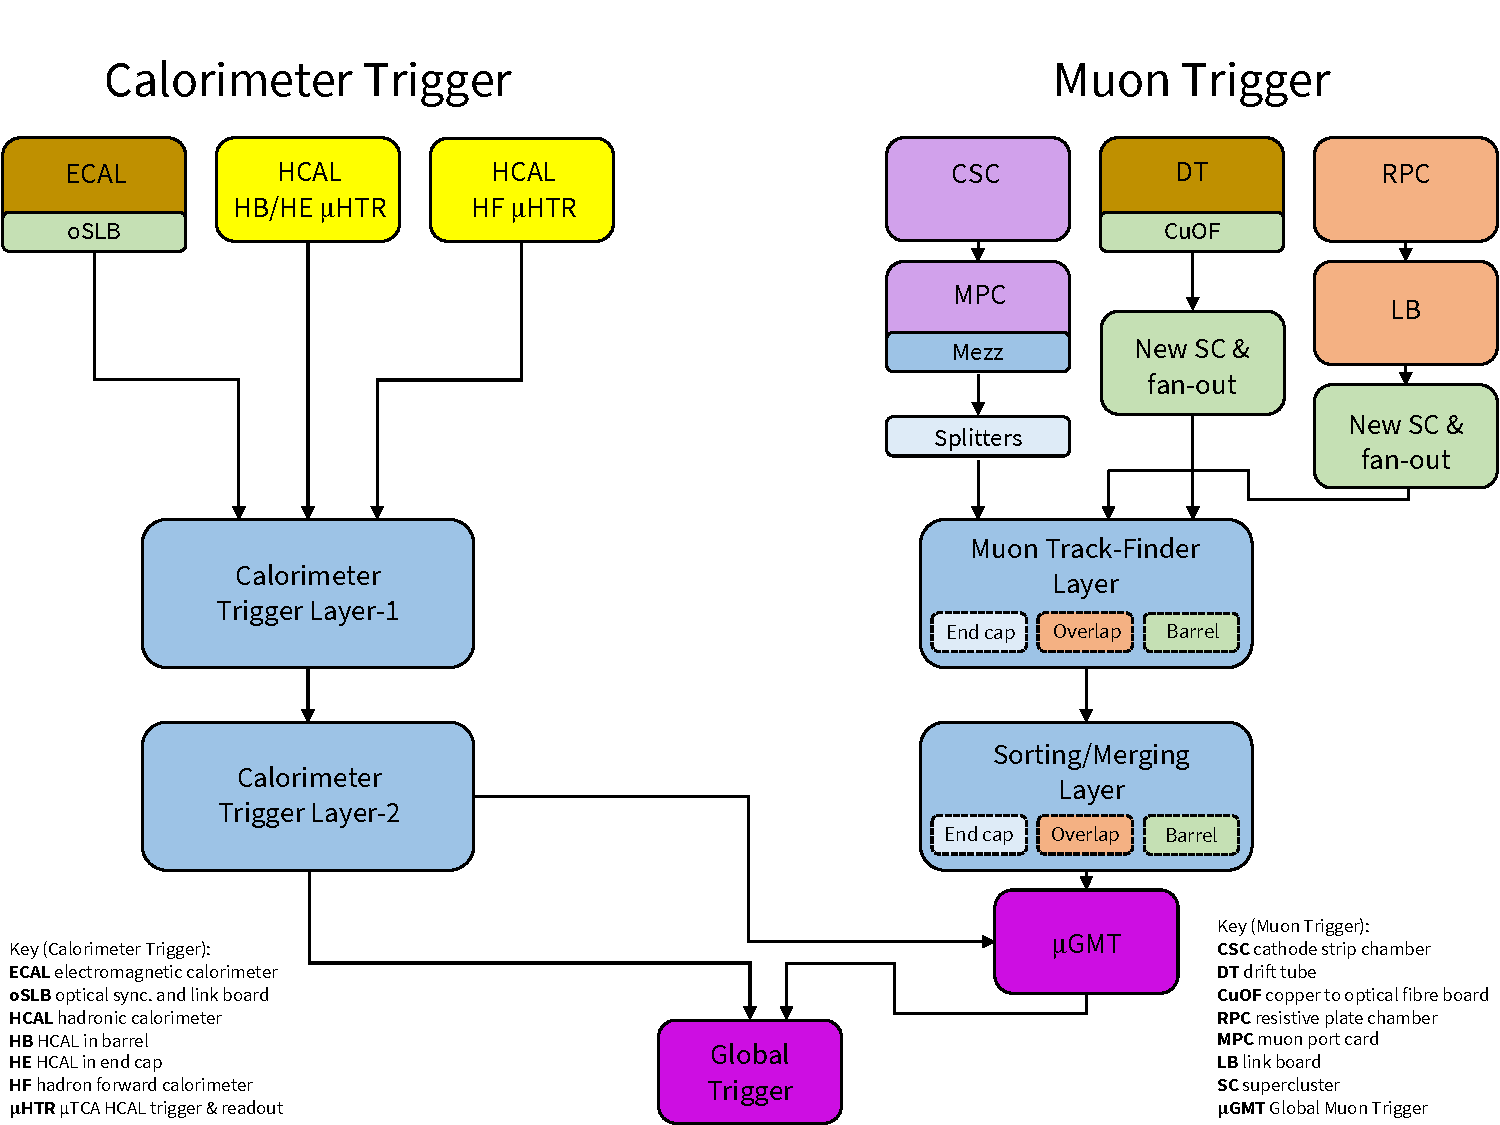
\includegraphics[width=0.75\textwidth]{figures/CMS_L1T_data_flow_key_ordered.pdf}
    \caption[A summary of the CMS Level-1 Trigger data flow from the hits recorded by the subsystems to the Global Trigger]{A summary of the \acrshort{cms} \acrlong{l1t} data flow from the hits recorded by the subsystems to the Global Trigger. Figure reproduced from Ref.~\citenum{Dev_2017}.}
    \label{fig:cms_l1t_data_flow}
\end{figure}

A small subset of data from the \acrshort{l1t} is diverted for monitoring purposes. During data taking periods, \acrshort{cms} has a plethora of members that participate in the supervision and maintenance of the experiment. At Point 5, shifters monitor the different domains, collecting information from various sources. Data acquisition, data quality, access to the experimental cavern, the \acrshort{l1t} (which I have performed on numerous occasions), and the \acrshort{hlt} are among them. Experts in these, and more specific systems, are on call on a rotating period. I, myself, have been an on call for Layer-2 of the Calorimeter Trigger several times.


%=========================================================


\subsubsection{The High-Level Trigger}
\label{subsubsec:detector_hlt}

Events that pass a logical \texttt{OR} of the triggers at \acrlong{l1} are transmitted to the \acrshort{hlt}. The higher resolution data collected at the point of collision is available, along with information from the tracker. Populated with Intel Xeon processors (high core count CPUs), approximately 22,000 cores are available (by the end of Run-2) to process the data sent from the \acrshort{l1t}. In order to avoid a back-log, a 100\,kHz input rate allows a \acrshort{hlt} node $\sim$220\,ms to make a decision. High-level software in the \acrshort{cmssw} environment (written in C\texttt{++} and Python, see Chpt.~[REF]) % reference analysis tools/software section
is executed. A larger and more complex trigger menu is available, including the possibility analysis-specific triggers (such as those that target \acrshort{vbf} topologies in Chpt.~\ref{chap:higgstoinv}). Complex variables such as \alphaT can even be calculated and triggered on.

Physics objects are reconstructed further, with algorithms such as \glssymbol{antikt} used to cluster \glspl{jet}~\cite{Cacciari:2008gp}. Additional classification algorithms are also applied to objects, such as the \deepcsv neural network~\cite{Sirunyan:2017ezt} to identify \glspl{bjet}. A global event reconstruction from the \gls{particleflow} (\acrshort{pf})~\cite{CMS-PAS-PFT-09-001,CMS-PRF-14-001} is performed as well. Some of these algorithms can be computationally expensive. Consequently, only approximations/parametrisations are used at \acrshort{hlt} level. The full-scale versions of these kind of algorithms are re-run on the retained events in later stages of postprocessing.\footnote{If more detail is required here, I should make a separate subsubsection and discuss.}

The \acrshort{hlt} reduces the event rate from the maximum 100\,kHz input substantially to around 1\,kHz. The data stream of $\order{\text{6\,GB\,s}^{-1}}$ is then subject to further processing before the analysts access it. As well as the data being stored on networked hard drives at sites across the globe, back ups are made to magnetic tape for long term storage. As with the \acrlong{l1t}, some data is redirected for monitoring, object calibrations, and alignment of detector components.

% CMS Computing TDR: \cite{Bayatyan:838359}. See the Offline Data Preparation slides in the Induction Course folder. If computing/offline data prep. warrants its own subsubsection, add it.


%=========================================================


\subsubsection{Data reduction and compression}
\label{subsubsec:cms_data_tiers}

Several data ``tiers'' are used in \acrshort{cms} to serve different purposes. All sorted in \ROOT file containers,\footnote{Event and ancillary data are stored in tree structures (otherwise known as \emph{ntuples}), with ``branch'' and ``leaf'' levels that contain more specific quantities such as muon \pt, or \gls{jet} $\eta$.} RAW data is repacked straight from prompt reconstruction. The files are then converted to the RECO tier where objects are fully reconstructed. Files are large (around 1.3--1.4\,MB per event) and usually only kept for a short period of time for detector-related studies. The subset designed for analysis is designed \acrfull{aod}. However, the level of compression is not ideal, especially with the volume of data amassed in Run-2. This is why miniAOD was developed. By ``slimming'' the trees in the files (removing unnecessary branches) and using smaller numeric data types, the footprint is roughly 10--15\,\% that of \acrshort{aod}.

An even more drastic reduction was made possible by the introduction of the nanoAOD tier. The methods used to shrink \acrshort{aod} to miniAOD are applied more aggressively, and a flat tree structure (with only leaves, and no nested levels) is utilised for simpler access to data. This allows for much smaller file sizes $\order{\text{1--2\,kB}/\text{event}}$. Exporting to other data structures for integration with external libraries, such as \textsf{numpy} and \textsf{pandas}, is also achievable. While nanoAOD is unable to cover all analyses because of its reduced event content, it is suitable in our search for invisibly decaying Higgs bosons.


%=========================================================


\subsection{Simulating CMS data}
\label{subsec:cms_mc}

Data recorded by \acrshort{cms} is paramount for analyses searching for new physics. However, simulated samples are also of high importance. Events for specific processes are generated using \acrfull{mc} random sampling, and the output datasets are often collectively referred to by the method---``\acrlong{mc}'' or ``\acrshort{mc}.'' The datasets are often generated with large numbers of events to minimise the associated statistical uncertainty. \acrshort{mc} samples are useful in a variety of cases: understanding the kinematics of signal processes in searches for new physics, modelling background processes that can mimic signal, and comparisons to data for validation purposes.

A matrix element generator such as \madgraph~\cite{Alwall:2014hca} or \POWHEG~\cite{Nason:2004rx,Frixione:2007vw} models the hard scattering process, usually at \acrfull{lo} but sometimes at higher orders. Events then pass through a hadroniser (usually \PYTHIA~\cite{pythia82} in \acrshort{cms}) to model hadronisation of quarks and gluons, sometimes known as the \emph{parton shower}---the softer radiation that accompanies the hard scatter. \Glspl{jet} are clustered here by, for example, the \gls{antikt}. The particles are also run through a detector simulation that emulates the configuration and response of the detector in different years. Material interactions and emulation of the triggers are included. \GEANTfour~\cite{AGOSTINELLI2003250,1610988,ALLISON2016186} provides this in \acrshort{cms}. Once the particles have been appropriately simulated, they are given the same postprocessing treatment as actual data, such as executing object-tagging algorithms so that the data and simulated samples are as comparable as possible.


%=========================================================


\subsection{Jet energy corrections in the Level-1 Trigger}
\label{subsec:detector_jecs}

Recording the properties of hadrons that are amalgamated into \glspl{jet} is not always consistent across the detector. While the components go through quality control, there is inevitably some variation in their performance. They can degrade at different rates. Some may also receive hits more often than others and be subject to greater radiation damage. As a result, non-uniformity of the detector response---as functions of \pt and $\eta$---must be compensated for. For \glspl{jet}, this comes in the form of \gls{jec}.

As outlined in Chpt.~\ref{subsubsec:detector_l1t}, the trigger primitives from the \acrshort{ecal} and \acrshort{hcal} enter Layer-1 of the Calorimeter Trigger, where coarse position- and energy-dependent calibrations are applied. Objects such as \glspl{jet} are initially identified in Layer-2, and preliminary calibrations correct their energy. Disregarding these, even at this early stage in the data acquisition workflow, can affect the efficiency and rate of the \acrlong{l1t}. It is therefore important to re-derive the calibrations regularly, since the configuration of the detector and beam conditions change over the lifetime of the experiment.

When a new round of calibrations are derived, there are many steps before this one. Preceding it, Layer-1 experts calculate their scale factors for the calorimeter towers. Once performed, the \acrlong{jec} are then derived in \acrshort{cmssw}. From early 2017 to mid-2018, I was responsible for procuring the \acrshort{jec}. The repository is accessible at \url{https://github.com/eshwen/L1JetEnergyCorrections}.\footnote{Note: I have only forked it from the original developers and made modifications on top.}


%=========================================================


\subsubsection{The procedure}
\label{subsubsec:detector_jec_procedure}

\acrshort{qcd} multijet \acrshort{mc} datasets with a large \pt range used to derive the Layer-1 and Layer-2 calibrations. Corresponding \glspl{jet} in data for this process can often be mismeasured (so providing good calibrations in the most difficult scenario is a good test), and \acrshort{mc} events contain ``truth-level'' information from the generator. Ntuples are made from these which have the Layer-1 corrections applied. Referring to the processing chain in Chpt.~\ref{subsec:cms_mc}, the \glspl{jet} these calibrations are derived for are post--hadronisation, but before interaction with the detector. They will be referred to as ``\acrfull{l1} \glspl{jet}.'' The reference \glspl{jet} directly from the generator (``GenJets'' as colloquialised in \acrshort{cms}) are important for matching to our \acrshort{l1} \glspl{jet} to ensure we are not mistakenly using \glspl{jet} from the parton shower that have no well-defined source.

The reference and \acrshort{l1} \glspl{jet} are matched using the variable $\Delta R$ (see Eq.~\ref{eq:delta_r}). The algorithm used to match the \glspl{jet} does so by inspecting each \acrshort{l1} \gls{jet} in descending \pt and searching for a reference \gls{jet} with $\Delta R < \text{0.25}$. If there is more than one match, the reference \gls{jet} with the smallest $\Delta R$ is taken. Then the next \acrshort{l1} jet (and so on) follows the same procedure, with the previous reference \gls{jet} removed from the matching collection.

The pairs of \glspl{jet} are categorised into sixteen bins of \abseta, the highest granularity available since the calibrations must run quickly on hardware. Each bin is then analysed in turn. Within each \abseta bin, the \gls{jet} pairs are subdivided into bins of the transverse momentum of the reference \gls{jet} (\ptRef).\footnote{Should I add tables somewhere of the \ptRef and \abseta bins for the calibrations?} The bin widths, like \abseta, are variable. The ratio of the transverse momentum of the \acrshort{l1} \gls{jet} (\ptLOne) to \ptRef is taken for each pair of \glspl{jet}. Our metric for measuring the detector response is the mean of these ratios:
\begin{equation}
    r_j = \expval{\ptLOne / \ptRef}
    \label{eq:jec_detector_response}
\end{equation}
The reciprocal of $r_j$ vs. \ptLOne is inspected and a correction curve is fitted. A gaussian captures the peak at low \pt and the following equation\footnote{Go into more detail regarding the equation? Reasoning, etc.} is used for the tail:
\begin{equation}
    \ptsup{{\mathrm{L1, \ corr.}}} = \ptLOne \cdot \left( p_0 + \frac{p_1}{ \left(\log_{10} \ptLOne \right) ^2 + p_2 } + p_3 \cdot \exp(-p_4 \left( \log_{10} \ptLOne - p_5 \right)^2) \right)
    \label{eq:corr_curve_jec_tail}
\end{equation}
The input parameters for the function may not be adequate for all cases, so they are often tuned to capture the low-\pt spike and high-\pt plateau (see Fig.~\ref{fig:detector_jecs_corr_curves} for an example). The value of this fit function in each \ptRef bin is exported.

% Should I note the pt_ref and abseta bins for the calibrations? In most recent talk in L1T DPG meetings/, I have the eta bins (also in iEta). In the sets of plots I have, I can probably also make a table of the pt_ref bins

\begin{figure}[htbp]
    \centering
    \begin{subfigure}[b]{0.45\textwidth}
        \includegraphics[width=\textwidth]{./figures/jecs/corrCurveBarrel.pdf}
        \caption{$0.435 < \abseta < 0.783$ (Barrel)}
        \label{fig:detector_jecs_corr_curve_Barrel}
    \end{subfigure}
    \hfill
    \begin{subfigure}[b]{0.45\textwidth}
        \includegraphics[width=\textwidth]{./figures/jecs/corrCurveHF.pdf}
        \caption{$4.191 < \abseta < 5.191$ (\acrshort{hf})}
        \label{fig:detector_jecs_corr_curve_HF}
    \end{subfigure}
\caption[Examples of correction curves used to calibrate the jet energies in two \abseta bins]{Examples of correction curves used to calibrate the \gls{jet} energies in two \abseta bins. The reciprocal of the response is plotted against the \pt of the \acrlong{l1} \gls{jet}, and a complex function (Eq.~\ref{eq:jec_detector_response}) fits the points. These plots are from the \acrlong{jec} performed on 2018 \acrshort{qcd} \acrlong{mc}.}
\label{fig:detector_jecs_corr_curves}
\end{figure}

Once all \abseta bins have been inspected, the calibrations are consolidated in several forms. A machine-readable lookup table is included in the firmware of the Layer-2 hardware, so that the corrections are applied in the trigger. A version is added to the \acrlong{l1t} packages in \acrshort{cmssw} so that the next steps in the calibration chain can utilise them.

A closure test is conducted to validate the corrections we have just produced. The \acrshort{mc} ntuples are regenerated with the \acrshort{jec} applied. \Gls{jet} matching is performed and the calibrations are checked. Many diagnostic and performance plots are produced to ensure the calibrations are functioning as expected. These can be inclusive of the number of \gls{pileup} interactions, or split into ranges to see if the calibrations differ between them. Examples of these are Fig.~\ref{fig:detector_jecs_scatter_BE} showing scatter plots of \ptRef vs. \ptLOne before and after \acrshort{jec} are applied, and Fig.~\ref{fig:detector_jecs_response} illustrating the response.

\begin{figure}[htbp]
    \centering
    \begin{subfigure}[b]{0.45\textwidth}
        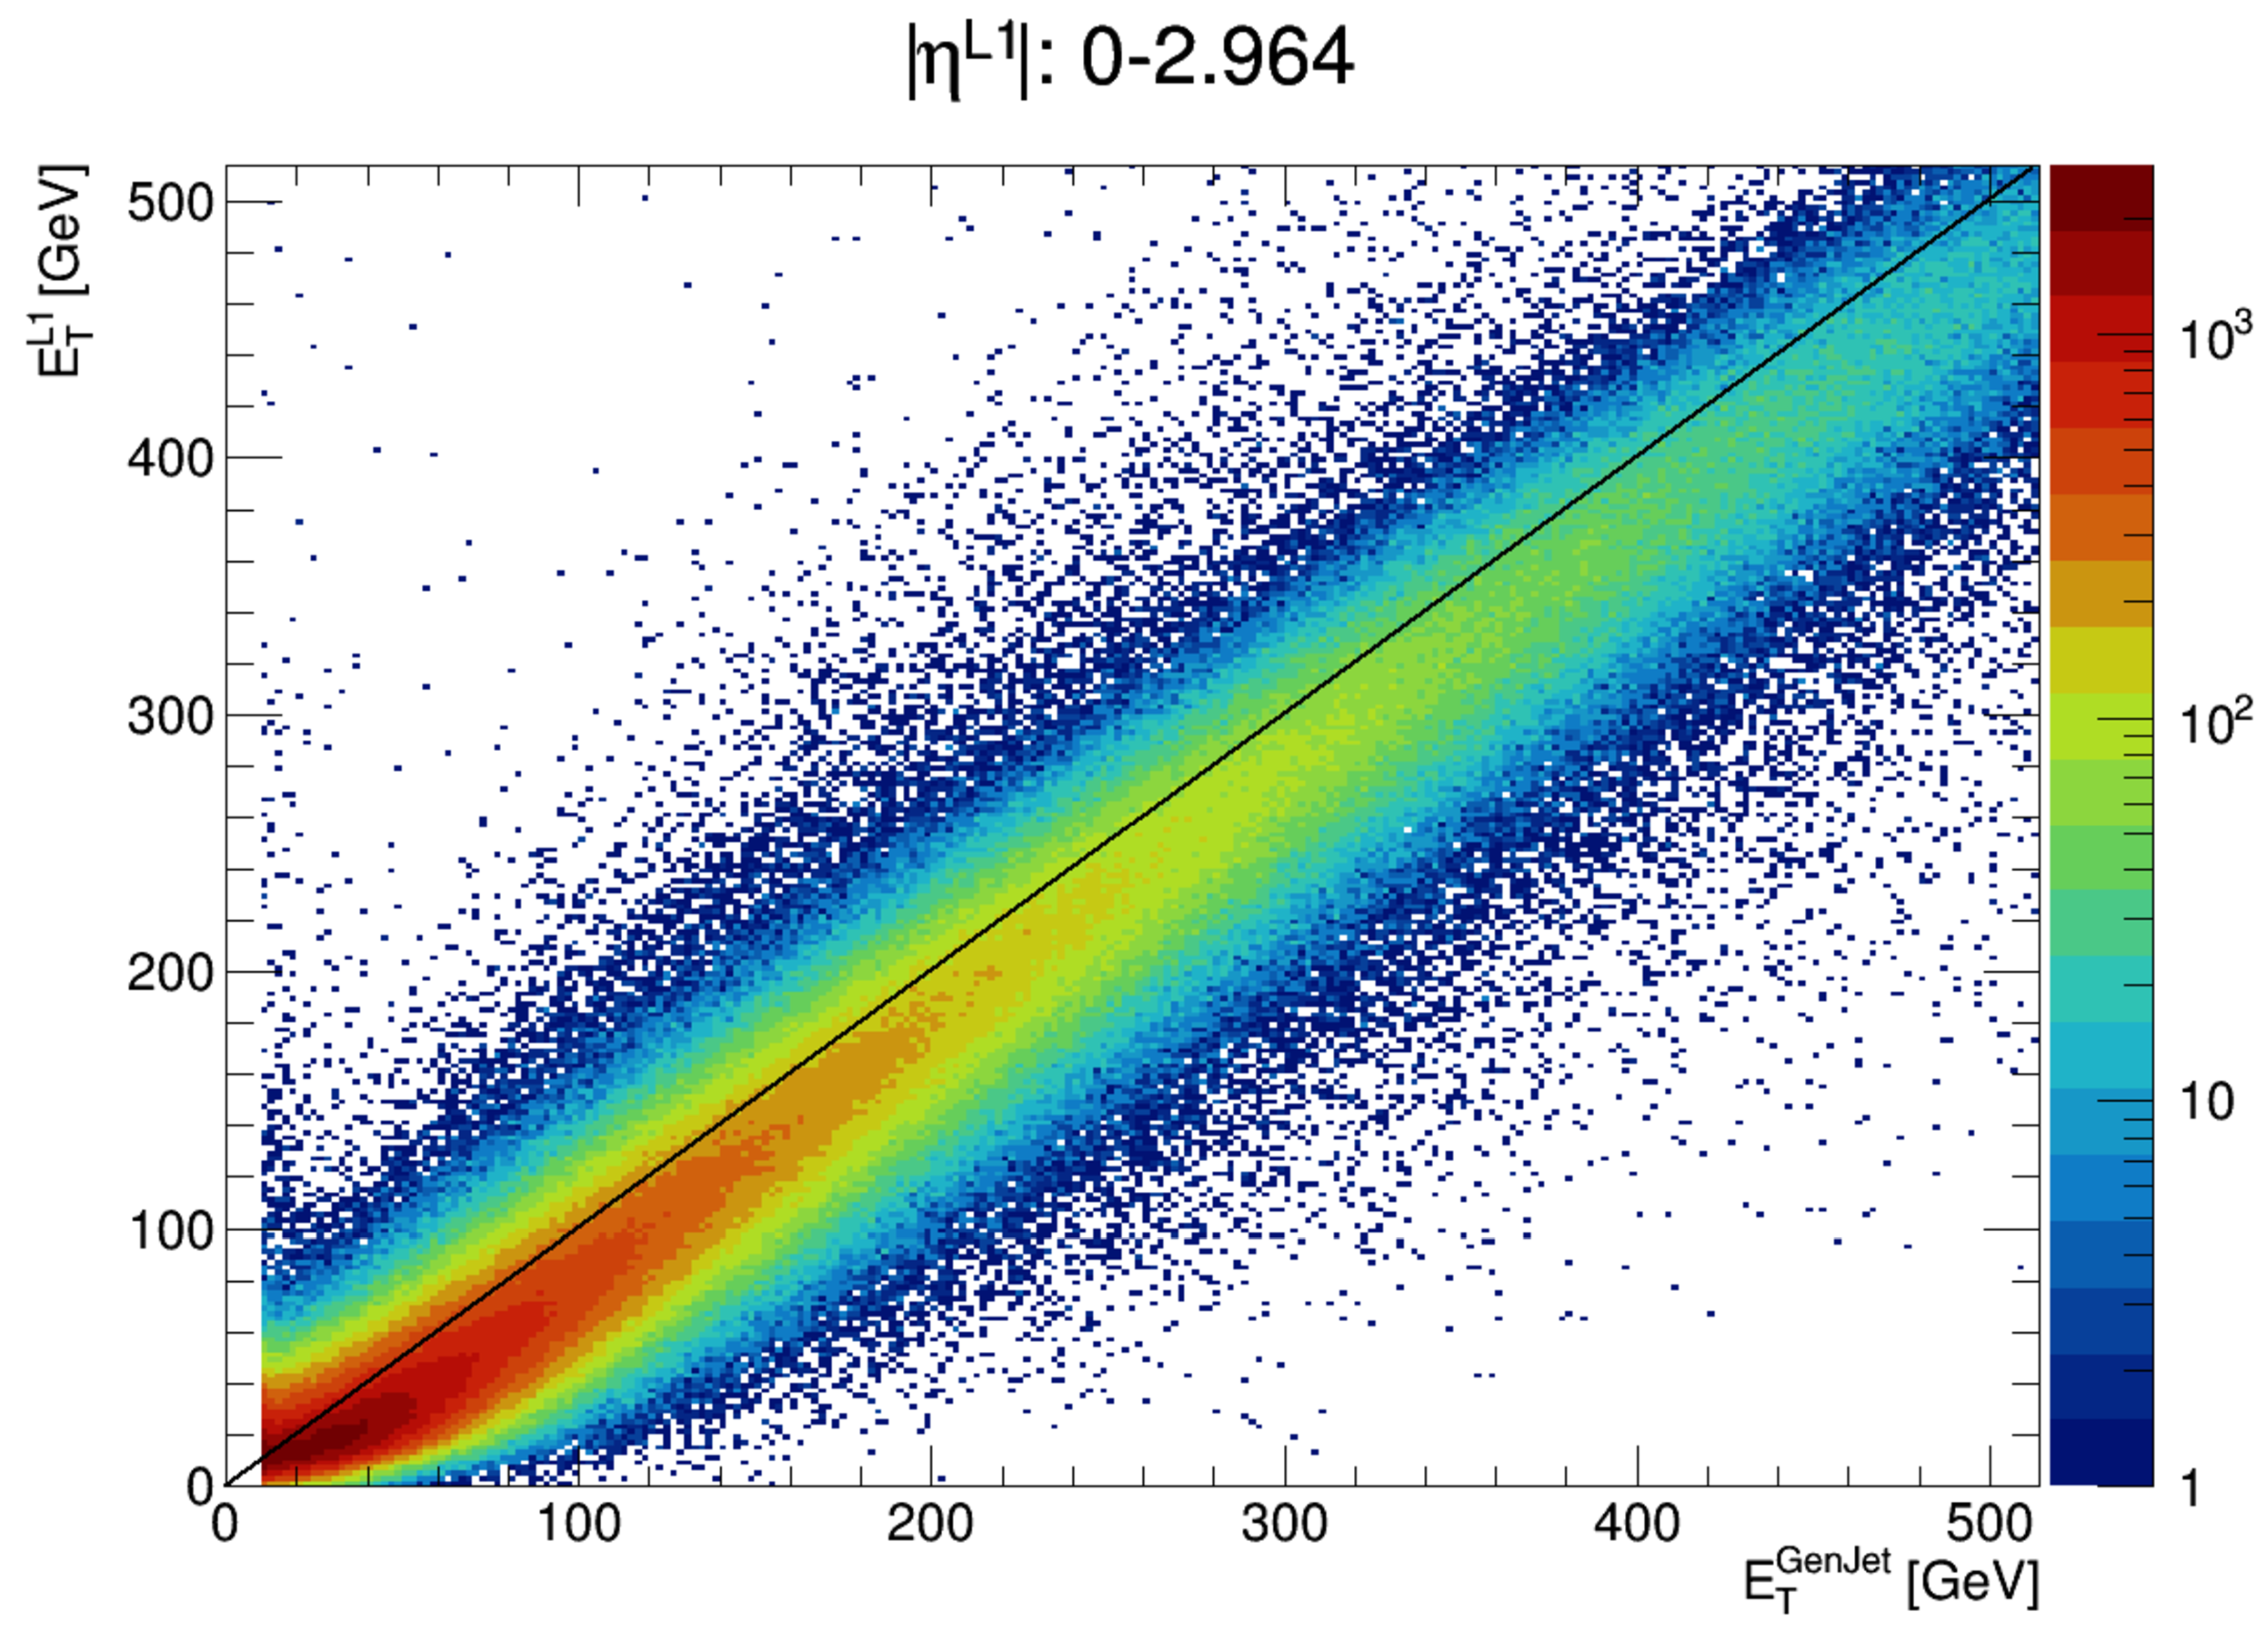
\includegraphics[width=\textwidth]{./figures/jecs/scatterPlotBeforeBE.pdf}
        \caption{Before corrections}
        \label{fig:detector_jecs_scatter_before_BE}
    \end{subfigure}
    \hfill
    \begin{subfigure}[b]{0.45\textwidth}
        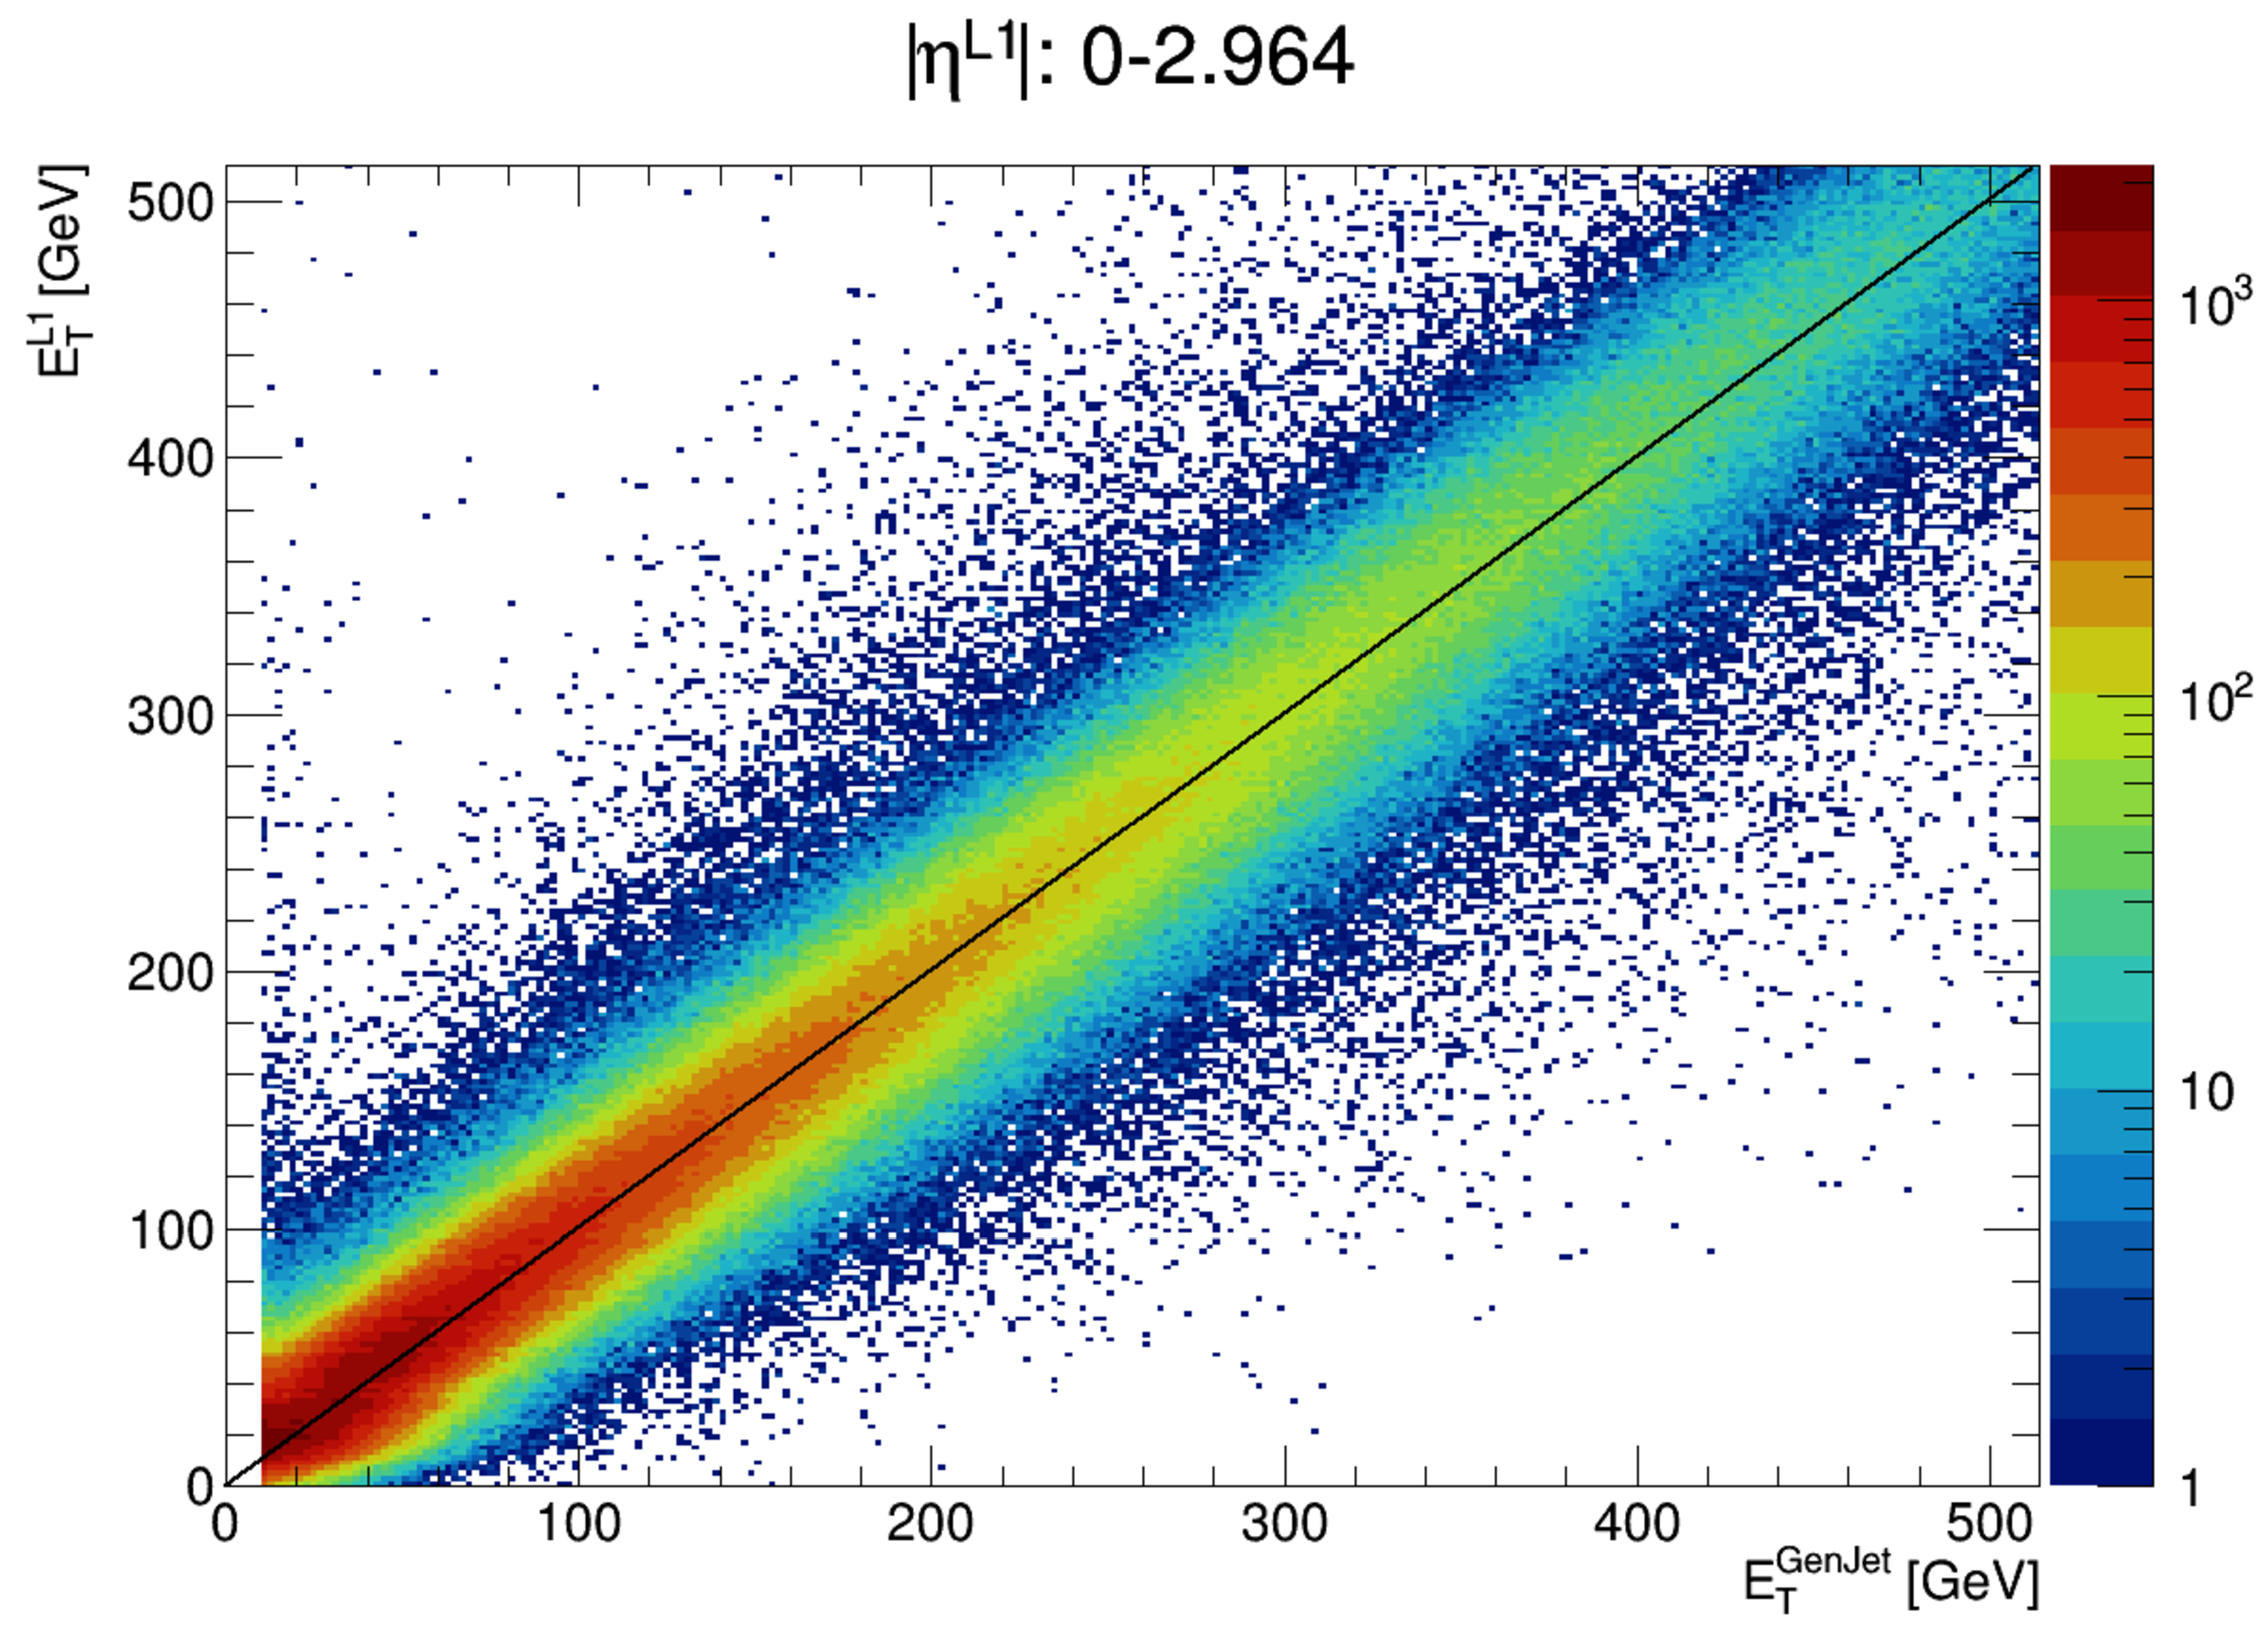
\includegraphics[width=\textwidth]{./figures/jecs/scatterPlotAfterBE.pdf}
        \caption{After corrections}
        \label{fig:detector_jecs_scatter_after_BE}
    \end{subfigure}
\caption[The energies of matched pairs of jets in the entire barrel and end cap, in the pileup 40--50 range, before and after jet energy corrections have been applied]{The energies of matched pairs of \glspl{jet} in the entire barrel and end cap, in the \gls{pileup} 40--50 range, before and after \acrlong{jec} have been applied. After calibrations, the distribution is much more symmetrical. An equivalent plot using \glspl{jet} from \acrshort{lhc} data is expected to look similar after applying these calibrations.}
\label{fig:detector_jecs_scatter_BE}
\end{figure}

\begin{figure}[htbp]
    \centering
    \begin{subfigure}[b]{0.45\textwidth}
        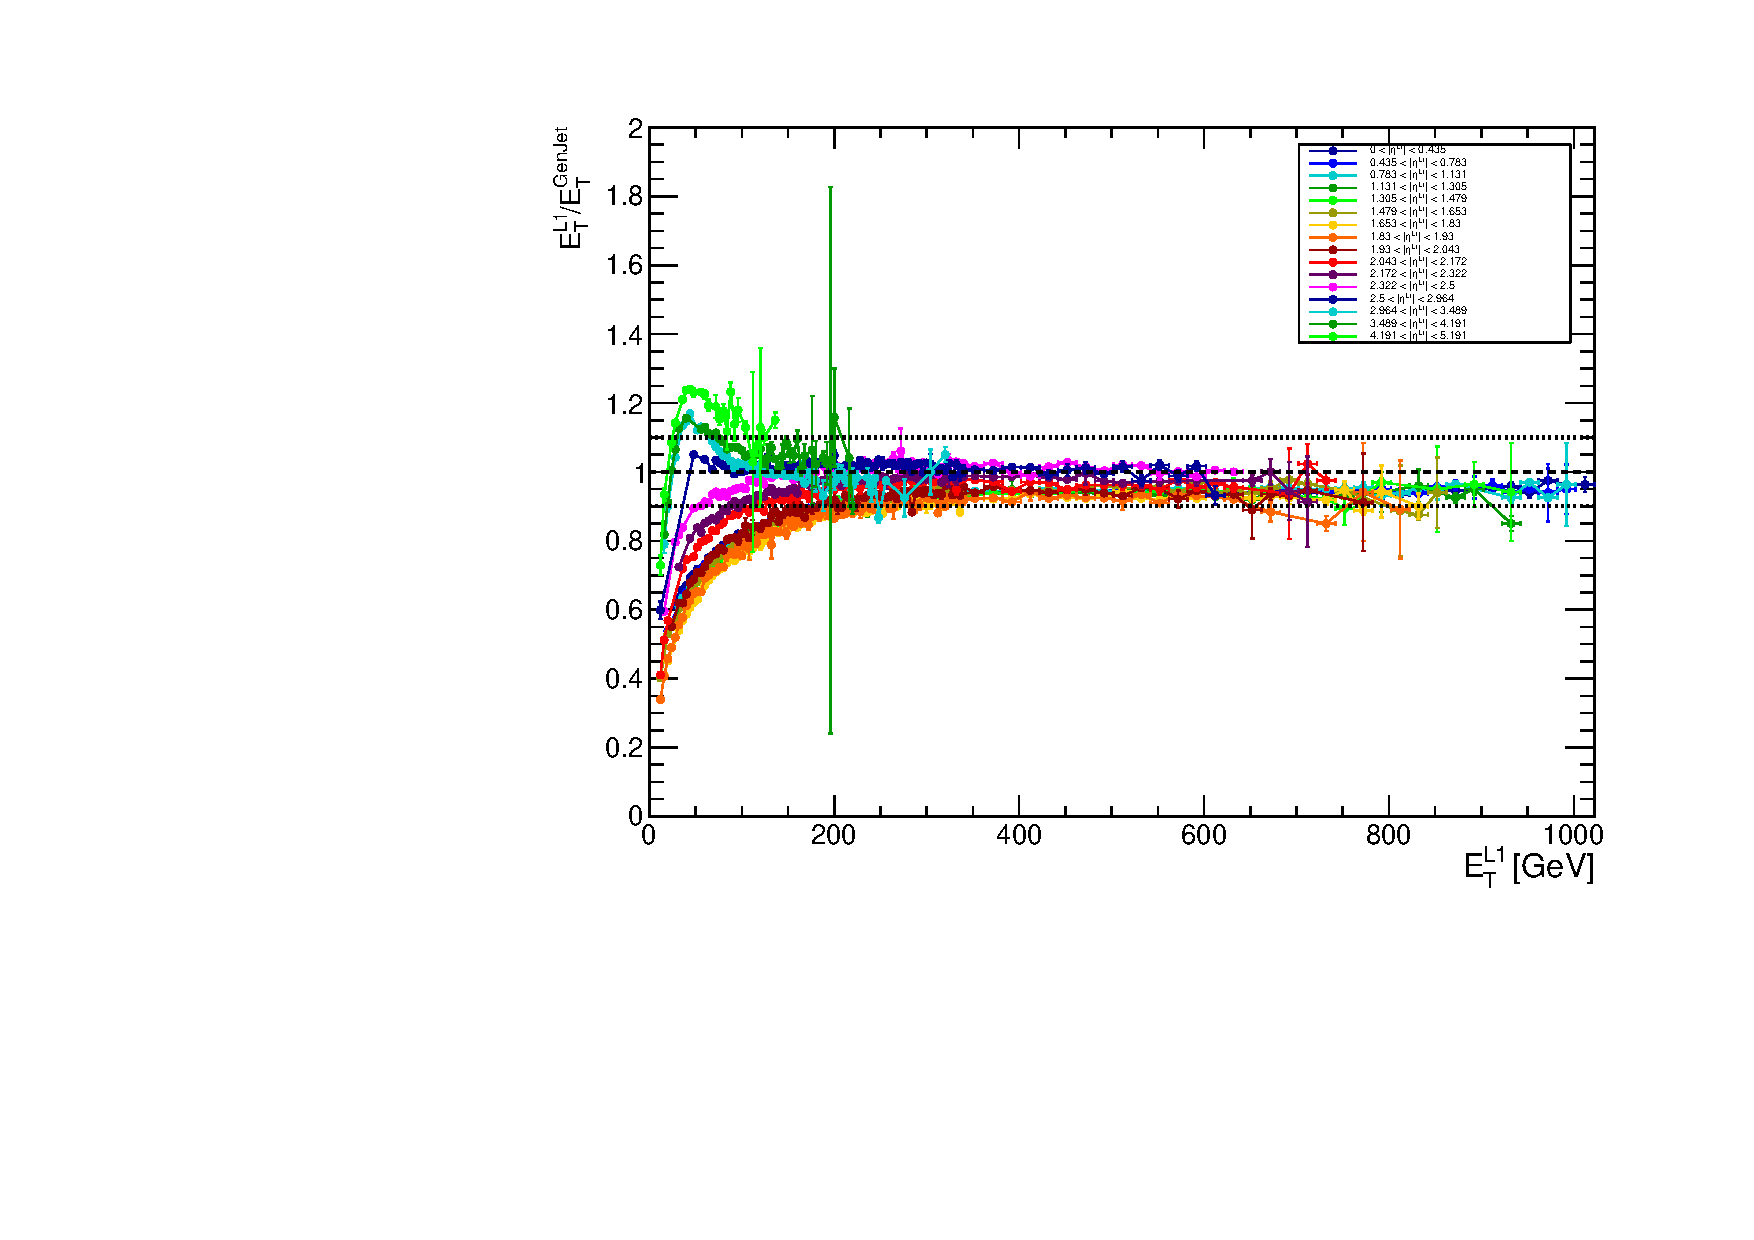
\includegraphics[width=\textwidth]{./figures/jecs/response_before.pdf}
        \caption{Before corrections}
        \label{fig:detector_jecs_response_before}
    \end{subfigure}
    \hfill
    \begin{subfigure}[b]{0.45\textwidth}
        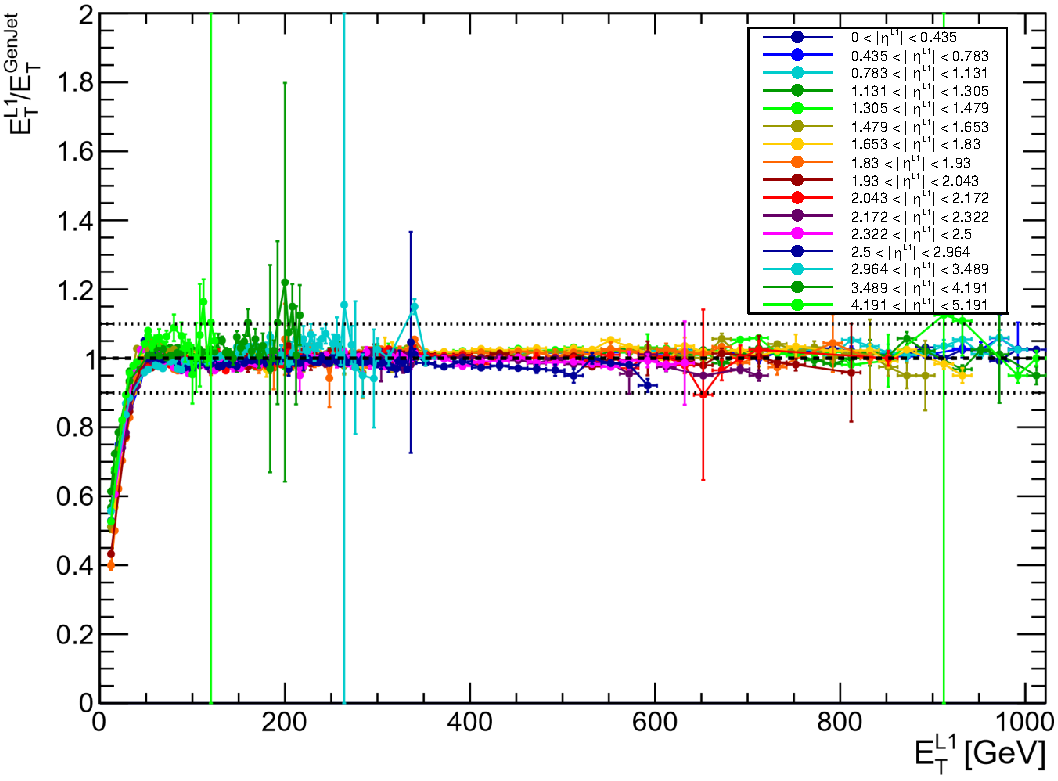
\includegraphics[width=\textwidth]{./figures/jecs/response_after.pdf}
        \caption{After corrections}
        \label{fig:detector_jecs_response_after}
    \end{subfigure}
\caption[The response curves in each \abseta bin as a function of \ptLOne, in the pileup 40--50 range, before and after jet energy corrections are applied]{The response curves in each \abseta bin as a function of \ptLOne, in the \gls{pileup} 40--50 range, before and after \gls{jec} are applied. Note that in panel b, the $x$-axis is the corrected \ptLOne.}
\label{fig:detector_jecs_response}
\end{figure}


%=========================================================
